\documentclass[english,12pt]{article}
\usepackage{blindtext} % Lorem ipsum
% Packages
\usepackage[a4paper,includeheadfoot,margin=2cm]{geometry} % Layout ,showframe
\usepackage{caption}
\usepackage[hidelinks]{hyperref} %links within the document and for clickable URLs
\usepackage{graphicx}
\usepackage[export]{adjustbox} % to beable to position images
\usepackage{amsmath} % equations

\usepackage[backend=bibtex,style=ieee]{biblatex} % or verbose-trad2
\bibliography{source.bib} % add sources to source.bib file
% https://www.latex-tutorial.com/tutorials/bibtex/

\usepackage{titling} % So you can use theauthor

\usepackage[hybrid]{markdown} % Used to convert markdown
% pdflatex --shell-escape
%https://www.overleaf.com/learn/latex/Articles/How_to_write_in_Markdown_on_Overleaf

%Bild
\graphicspath{{img/}}
\usepackage{float} % Allows putting an [H] (place HERE & not where LaTeX wants to put)

\usepackage{fancyhdr} % Header & Footer

% Für Deutsch
%\usepackage[utf8]{inputenc}
%\usepackage[ngerman]{babel} --- für deutsh

\usepackage{siunitx} % Required for alignment
\sisetup{
	round-mode          = places, % Rounds numbers
	round-precision     = 2, % to 2 places
}
\usepackage{booktabs} % For prettier tables

% TODO: better Title page
% Document information
\title{ZHAWo - Platform Independent Timetable App}
\author{Bachmann Dominik, Visser Julian}

% Header & Footer
\pagestyle{fancy}
\fancyhf{}
\lhead{PA - HS 2018}
\chead{}
\rhead{ZHAWo}
\lfoot{}
\cfoot{\thepage}
\rfoot{}

\begin{document}

	% !TEX root = pa_doc.tex

%----------------------------------------------------------------------------------------
%	TITLE PAGE
%----------------------------------------------------------------------------------------
\begin{titlepage} % Suppresses displaying the page number on the title page and the subsequent page counts as page 1
	\newcommand{\HRule}{\rule{\linewidth}{0.5mm}} % Defines a new command for horizontal lines, change thickness here

	\center % Centre everything on the page

	%------------------------------------------------
	%	Headings
	%------------------------------------------------

	
\includegraphics[width=0.3\textwidth, left]{./assets/zhawLogo.jpeg}\\[1cm]

	\textsc{\Large Projekt Arbeit}\\[0.5cm] % Major heading such as course name

	\textsc{\large HS 2018}\\[0.5cm] % Minor heading such as course title

	%------------------------------------------------
	%	Title
	%------------------------------------------------

	\HRule\\[0.5cm]

	%------------------------------------------------
	%	Logo
	%------------------------------------------------

	
\includegraphics[width=0.4\textwidth]{./assets/zhawoLogo.png}\\[0.5cm]

	\textsc{\large \textbf{ZHAWo} \\[0.2cm]
									--- \\[0.3cm]}
	% Title of your document
	\textsc{\large Platform Independent Timetable App}\\[0.5cm]


	\HRule\\[1cm]

	%------------------------------------------------
	%	Author(s)
	%------------------------------------------------

	\begin{minipage}{0.4\textwidth}
		\begin{flushleft}
			\large
			\textit{Authors}\\
			Bachmann Dominik \\
			Visser Julian % Your name
		\end{flushleft}
	\end{minipage}
	~
	\begin{minipage}{0.4\textwidth}
		\begin{flushright}
			\large
			\textit{Supervisor}\\
			Meier Andreas % Supervisor's name
		\end{flushright}
	\end{minipage}

	%----------------------------------------------------------------------------------------

	%------------------------------------------------
	%	Date
	%------------------------------------------------
	\vfill
	{\large\today} % Date, change the \today to a set date if you want to be precise

\end{titlepage}


	\pagenumbering{gobble}


	%Index
	\newpage
	\pagenumbering{roman}
	\tableofcontents
	\newpage
	%Abstract
	% !TEX root = pa_doc.tex
\begin{abstract}
\begin{markdown}

\noindent Where is my next lecture? Is there a free room for me to study in? What is the Lunch Menu today?

\noindent These are just a few of the many questions Students have to deal with daily and getting an anwser to these questions isn't always that easy.

\noindent Our vision for zhawo is to solve this. All the information regarding your life a the ZHAW in one place.

\noindent We want to provide our Users a fast, Reliable and Engaging experience across all Platforms. That is why we have chosen to develop zhawo as a Progressive Web App. Progressive Web Apps are web apps that behave like native apps. That means the application can be accessed by any device that has a browser, whilst still gives the user the look and feel of a native app.
\end{markdown}
\end{abstract}


	% Main body of your document
	\newpage
	\pagenumbering{arabic}

	%\markdownInput{example.md}

	%Introduction
	% !TEX root = pa_doc.tex
\begin{markdown}

# Introduction

## Goals

Students of the Zurich University of Applied Sciences (ZHAW) have to visit multiple websites or use different applications on a daily basis in order to get information about their schedule, the offered menus in their campus mensa and events organized by the Verein Studierende ZHAW (vszhaw).

For their schedule, a student can either visit the official site \cite{DUMMY} or use the official application for either Android \cite{DUMMY} or iOS \cite{DUMMY}. The official site was designed for use on desktop browsers and is not optimized for responsiveness and display on phones. And while the official Android application is well maintained and offers a lot of additional features - such as direct access to public transport timetables and mensa menu plans - its iOS counterpart lacks many of these additional features and looks and feels rather unpolished in comparison. This difference in quality and features is a common occurence because the development of native applications requires two seperate code bases for Android and iOS \cite{DUMMY}. The most glaring issue with the iOS application is the lack of offline functionality. When a user network cuts out, even schedule information that is previously loaded can no longer be access after navigating away.

When students want to check the mensa menus of their campus, they have the option of visiting the SV groups site or use the official Android or iOS application. These options suffer from the same issues as previously explained for the schedule.

With ZHAWo, our goal is to provide students with an improved application to have access to their schedule and mensa menus in one single cross-platform application. Additionally, with ZHAWo students can search for unoccupied rooms. This functionality was - until about two years ago - provided by an Android application that was no longer maintained and eventually disappeared from the Google Play Store. While the study rooms at for example the Technikum campus offer a space for both quiet work as well as group projects, in our experience as students it was very convenient to have a service to quickly look up free rooms without having to walk from room to room. Another feature ZHAWo provides is the integration of news and events of the vszhaw directly into the application. We aim to reduce the effort that is needed to stay up to date with the vszhaw and hope that both students and the vszhaw can profit from this.

By using Progressive Web Application (PWA) technologies \cite{DUMMY} in combination with JavaScript frameworks for both front- and backend, we achieve a consistent user experience throughout desktop devices and both Android and iOS applications. We eliminate the issue of having to maintain seperate code bases for different platforms while still being able to provide a native feel and functionality. PWA features such as offline caching of HTTP requests allow us to overcome previously mentioned issues with reliability on spotty networks.

An additional advantage we gain by using PWA technologies and the same programming language across the full stack is fast prototyping in an agile development process. Development of additional features and functionality can be achieved at a much faster rate with a single code base across all platforms.

\newpage

## Primary Functions

While our goal is to develop a feature rich application tailored to students of the ZHAW, we established the following four primary functions ZHAWo should provide in its prototype. Using an agile development approach, the scope of this project was to implement these primary functions in a prototype and adjust them to student feedback.

\begin{itemize}
  \item \textbf{Timetable}: A user can access their schedule and look up schedules of lecturers, classes, courses and rooms.
  \item \textbf{Menu plans}: A user can access menu plans of the different campus mensas across the ZHAW.
  \item \textbf{Room search}: A user can look for and find free rooms for a specified time-frame and location.
  \item \textbf{Student events}: A user can access vszhaw news and events to bring more attention to student parties and events.
\end{itemize}

After having established the core functionalities and a prototypical version of ZHAWo in the scope of this project, the features will be iteratively expanded and improved to end up with a production-ready application.

\end{markdown}


	%Architecture
	% !TEX root = pa_doc.tex
\begin{markdown}

% TODO: rename file

# Architecture

*add image*

## Frontend
For the presentation of the web application to the user, we used React\cite{React}. We decided to use React because of its potential to write cleaner code with component based modularity. To minimise potential problems and to insure a a unidirectional data flow we chose to incorporate  the flux pattern into the architecture design, instead of using the typical Model View Controller (MVC) architecture.

The data for the front end is provided by the back end RESTful API service and retrievable through HTTP calls. Each fetch request is cached using a service worker. We built the service worker using Workbox\cite{Workbox}. Workbox is a library that implements in a set of service worker best practices and helps you get the most out of your service workers.

### PWA
\say{Progressive Web Apps (PWA) are experiences that combine the best of the web and the best of apps.}\cite{WhatIsPWA}

Google and other companies have developed a new, modern web application standard. PWAs implement said standard and receive additional permission as a rewarded for doing so. This allows PWA to behave and feel like native apps. They live can on the user's home screen, offer a full screen experience, access device hardware (camera, GPS, etc) and can even re-engage users with push notifications\cite{PWA}.  When launched from the user’s home screen a Progressive Web App can load instantly, regardless of the network state. This is done by with the help of service workers.

#### Service Workers
A service worker is like a client-side proxy and that allows control of the cache. You can improve the loading speed of your page by pre-caching key resources. Using cache also eliminates the dependence on the network, ensuring a reliable offline experience for your users.\cite{ServiceWorker}

### React
React\cite{React} was originaly developed by Facebook and is one of the most popular UI librarys. It allows you to create reusable Compents using JSX, a syntax extension to JavaScript.
The idea behind React is to design simple views for each state of the application. Doing so allows it to only update and render components that need to be changed, thereby improving performance immensely.

#### Flux
Flux\cite{OurReadme} is a application pattern developed by Facebook. It's goal is to insure a a unidirectional data flow in React apps. The use of this practice enhances the quality and performance of the code by improving the data consistency. It is the optimal architecture for the use of React.

\begin{figure}[H]
  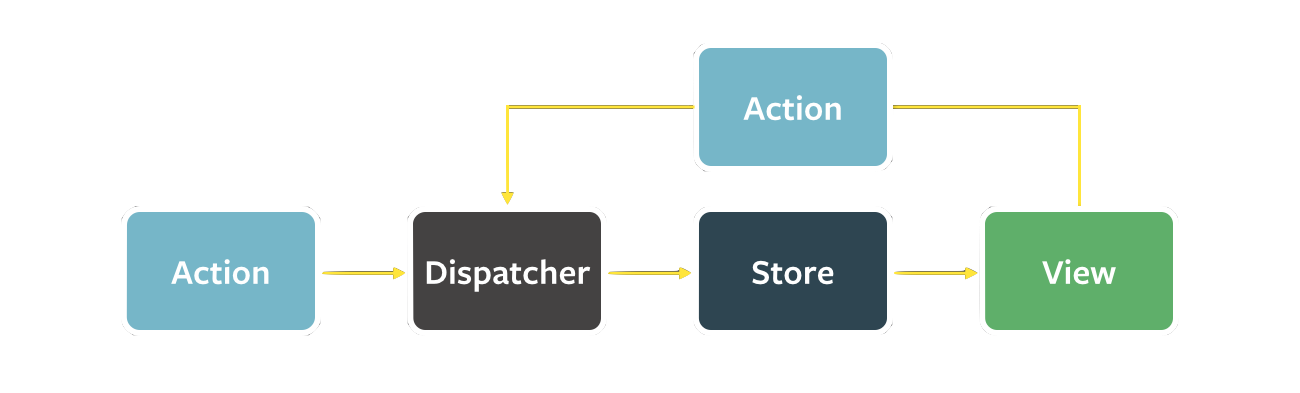
\includegraphics[width=10cm, center]{./assets/flux.png}
  \caption{Flux Model{\cite{FluxModel}}}
\end{figure}



% TODO: bild ref https://facebook.github.io/flux/img/flux-simple-f8-diagram-with-client-action-1300w.png

In Flux, the dispatcher is a singleton that directs the flow of data to ensure that updates do not cascade, which would lead to unpredictable behaviour. When a user interacts with a React view, the view sends an action through the dispatcher, which notifies the stores that hold the application’s data. When the stores change state, the view gets notified and changes accordingly.


## Backend
The Sever-side of ZHAWo is implemented in NodeJS\cite{Node}. We use the ExpressJS Server to handle all the API calls.

### NodeJS
Node.js is a JavaScript runtime environment, designed to build scalable network applications\cite{Node}.
*öpis vo da https://nodejs.org/en/about/* blocking and so on
#### Express
Express\cite{Express} is a minimal and flexible web application framework for Node.js. It provides HTTP utility methods and allows you to create a robust API.

% TODO: add image front-back api calls and stuff

% TODO: expand this, explain CampusInfo -> why we needed our own backend blabla

\end{markdown}


	%Discussion & Prospects
	% !TEX root = pa_doc.tex
\begin{markdown}

% TODO: rename file

# Architecture

*add image*

## Frontend
For the presentation of the web application to the user, we used React\cite{React}. We decided to use React because of its potential to write cleaner code with component based modularity. To minimise potential problems and to insure a a unidirectional data flow we chose to incorporate  the flux pattern into the architecture design, instead of using the typical Model View Controller (MVC) architecture.

The data for the front end is provided by the back end RESTful API service and retrievable through HTTP calls. Each fetch request is cached using a service worker. We built the service worker using Workbox\cite{Workbox}. Workbox is a library that implements in a set of service worker best practices and helps you get the most out of your service workers.

### PWA
\say{Progressive Web Apps (PWA) are experiences that combine the best of the web and the best of apps.}\cite{WhatIsPWA}

Google and other companies have developed a new, modern web application standard. PWAs implement said standard and receive additional permission as a rewarded for doing so. This allows PWA to behave and feel like native apps. They live can on the user's home screen, offer a full screen experience, access device hardware (camera, GPS, etc) and can even re-engage users with push notifications\cite{PWA}.  When launched from the user’s home screen a Progressive Web App can load instantly, regardless of the network state. This is done by with the help of service workers.

#### Service Workers
A service worker is like a client-side proxy and that allows control of the cache. You can improve the loading speed of your page by pre-caching key resources. Using cache also eliminates the dependence on the network, ensuring a reliable offline experience for your users.\cite{ServiceWorker}

### React
React\cite{React} was originaly developed by Facebook and is one of the most popular UI librarys. It allows you to create reusable Compents using JSX, a syntax extension to JavaScript.
The idea behind React is to design simple views for each state of the application. Doing so allows it to only update and render components that need to be changed, thereby improving performance immensely.

#### Flux
Flux\cite{OurReadme} is a application pattern developed by Facebook. It's goal is to insure a a unidirectional data flow in React apps. The use of this practice enhances the quality and performance of the code by improving the data consistency. It is the optimal architecture for the use of React.

\begin{figure}[H]
  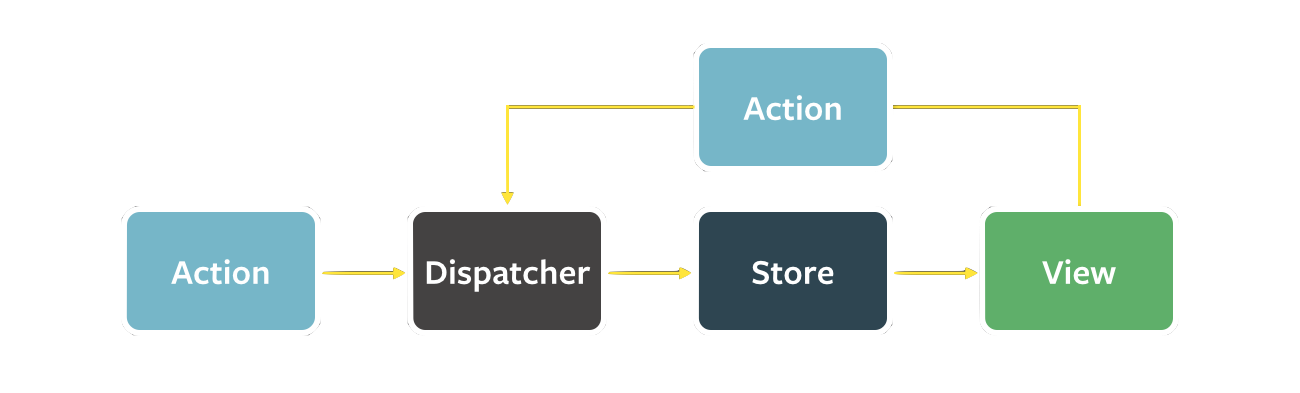
\includegraphics[width=10cm, center]{./assets/flux.png}
  \caption{Flux Model{\cite{FluxModel}}}
\end{figure}



% TODO: bild ref https://facebook.github.io/flux/img/flux-simple-f8-diagram-with-client-action-1300w.png

In Flux, the dispatcher is a singleton that directs the flow of data to ensure that updates do not cascade, which would lead to unpredictable behaviour. When a user interacts with a React view, the view sends an action through the dispatcher, which notifies the stores that hold the application’s data. When the stores change state, the view gets notified and changes accordingly.


## Backend
The Sever-side of ZHAWo is implemented in NodeJS\cite{Node}. We use the ExpressJS Server to handle all the API calls.

### NodeJS
Node.js is a JavaScript runtime environment, designed to build scalable network applications\cite{Node}.
*öpis vo da https://nodejs.org/en/about/* blocking and so on
#### Express
Express\cite{Express} is a minimal and flexible web application framework for Node.js. It provides HTTP utility methods and allows you to create a robust API.

% TODO: add image front-back api calls and stuff

% TODO: expand this, explain CampusInfo -> why we needed our own backend blabla

\end{markdown}



	\newpage

	\section{Appendix}

	\listoffigures
	\listoftables
	%\renewcommand\refname{Literaturverzeichnis}% rename --- für deutsh
	\printbibliography  % Uses source.bib to make ref table

\end{document}
